%%%----------------------------------------------------------
\chapter{SIFT-Based Image Stitching}
\label{chap:sift}
%%%----------------------------------------------------------

The goal of this assignment was to stitch a pair of images together by applying the SIFT method. 

\section{Algorithm}
A stitching algorithm consists of a few basic steps:
\begin{enumerate}
	\item Find distinctive points/features in the images.
	\item Establish correspondence between those sets of features (similar to what we did in assignment \ref{chapter:icp}).
	\item Calculate the transformation between these sets.
	\item Apply the transformation to one of the images.
\end{enumerate}

Some of these things were already implemented and included in the assignment. So the steps which needed to be done were:
\begin{enumerate}
	\item Extract the color images from an image stack and convert them to type FloatProcessor.
	\item Apply the \textit{SIFT detector} to both both images to detect \textit{SIFT features}. And we use a provided \textit{SiftMatcher} to find matching descriptors.
	\item We feed these matches into a provided \textit{projection mapper} called \texttt{ProjectiveMapping} which calculates the transformation matrix.
	\item This matrix is applied to one image and the other image is shown on top. The image intensities are merged by taking the average value which results in a semi transparent effect.
\end{enumerate}


\section{Pitfalls}
Since the mapper transforms the image without changing the size the size of the outcome has to be calculated and adjusted beforehand. Otherwise the pixels which get moved out of the frame are lost. The prevent this from happening the offset of the transformation was calculated in advance and if it exceeded the frame the image frame was adjusted. As soon as the frame size is correct the image is placed using the offset and the transformation is applied. The second image will be placed pixel by pixel on top of the transformed image.

\section{Results}
The results varied quite a lot between the different test images. While some pictures like figure \ref{fig:9_success} worked out really well others not at all (figure \ref{fig:9_fail}). It worked best if the images were taken out of the same picture (no change on viewing angle). If the viewing angle changed it resulted in artifacts shown in the stitched image like in figure \ref{fig:9_artifacts}. I tried to use another ProjectionMapper for the pictures which failed but the provided \texttt{HomographyEstimator} crashed when used with bigger images.

\begin{figure}
	\centering
	\frame{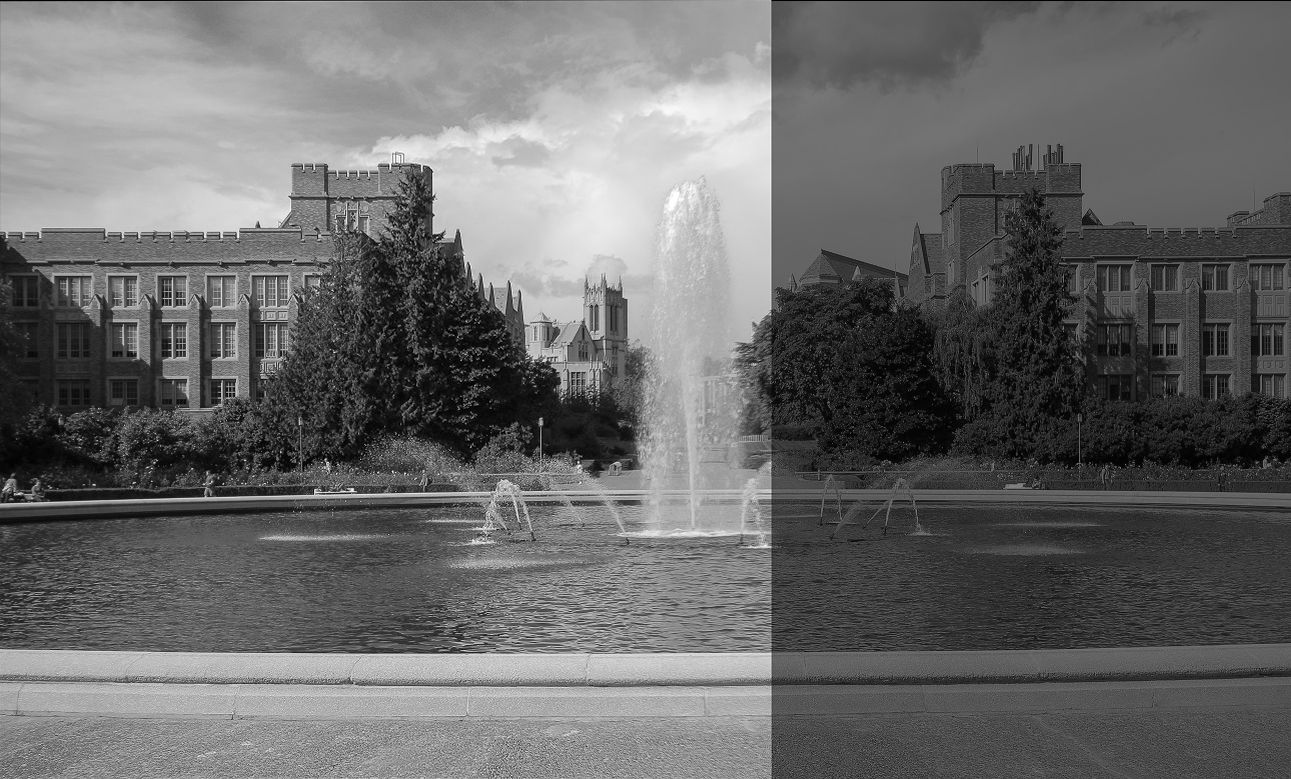
\includegraphics[width=0.8\linewidth]{images/washington3_stitched}}
	\caption{The \textit{Washington 3} test image was successfully stitched.}
	\label{fig:9_success}
\end{figure}

\begin{figure}
	\centering
	\frame{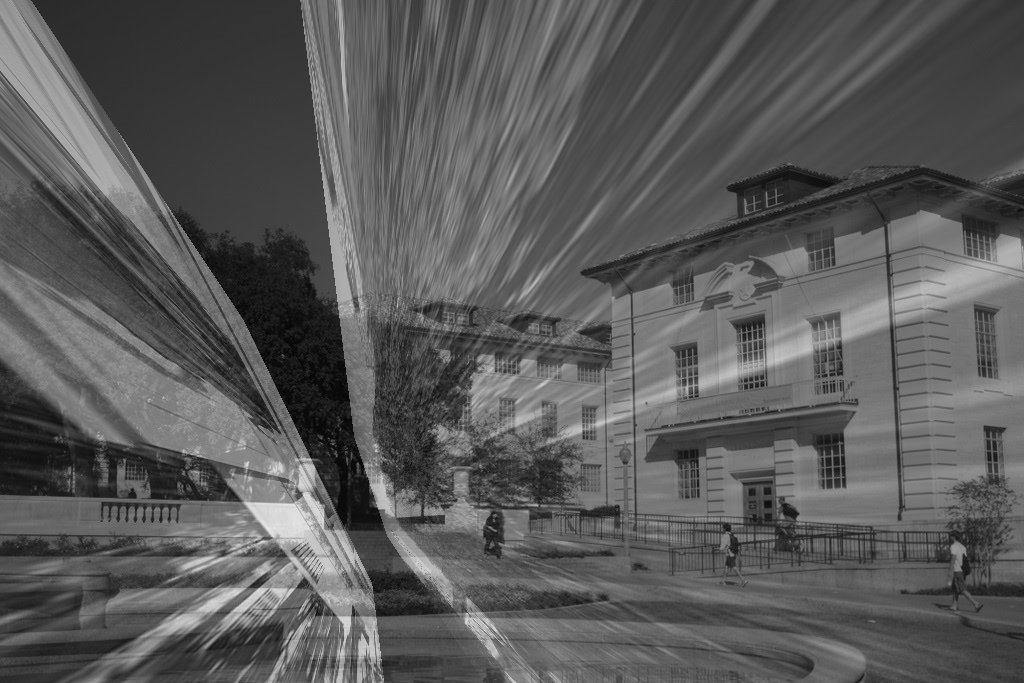
\includegraphics[width=0.8\linewidth]{images/washington1_stitched}}
	\caption{The stitching of the \textit{Washington 1} test image failed.}
	\label{fig:9_fail}
\end{figure}

\begin{figure}
	\centering
	\frame{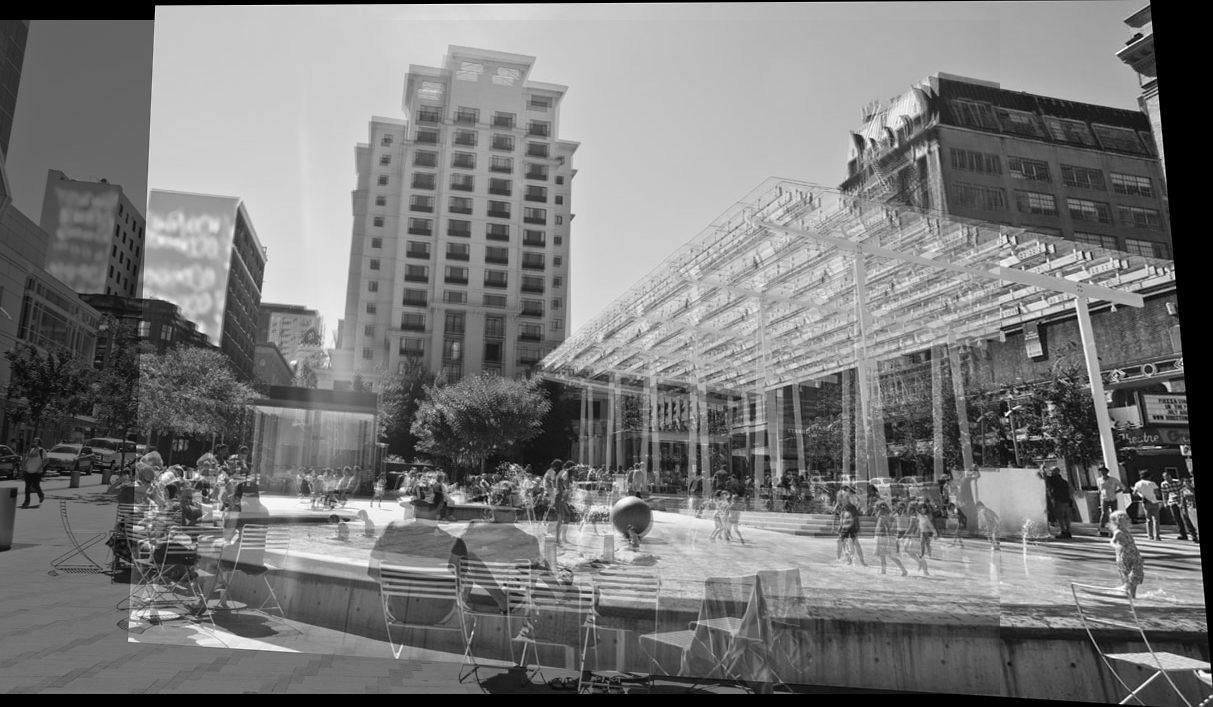
\includegraphics[width=0.8\linewidth]{images/fliu009_stitched}}
	\caption{The stitching of the \textit{fliu009} test image showed some artifacts due to the different viewing angles of the pictures.}
	\label{fig:9_artifacts}
\end{figure}